\chapter{Glossary}\label{appendix:glossary}

The following terms are used throughout this document.

\begin{description}
	\item[Asset] Something with a value. In the context of our application,
		an asset is a \textit{currency}. Often, this term is used in
		place of \textit{base currency}.
	\item[Backtesting] A process used to estimate the performance of a
		trading \textit{strategy} using historical \textit{market data}.
		Backtesting shows the results that a strategy would have
		achieved in the past.
	\item[Base currency] (or \textbf{Quoted currency}) Often called also
		\textit{asset}, is the \textit{currency} at the numerator of a
		\textit{market cross}.
	\item[Buy and Hold] (or \textbf{HODL}\footnote{\textit{Sic!} See:
		\url{https://en.wikipedia.org/wiki/Hodl}.}) The simplest
		\textit{strategy} possible: it opens a \textit{buy trade} at the
		start of the first \textit{trading day} and closes it at the end
		of the last candle. This strategy is often evaluated in
		comparison with other strategies, since a strategy that performs
		worse than the HODL strategy is totally useless.
	\item[Buy order] (or \textbf{Buy operation} or \textbf{Long order}) The
		action to buy the \textit{base currency} and sell the
		\textit{quoting currency} at the current \textit{market} price.
	\item[Buy trade] (or \textbf{Long trade}) A \textit{trade} where the
		\textit{entry order} is a \textit{buy order} (and thus the
		\textit{exit order} is a \textit{sell order} with the same
		\textit{amount}).
	\item[Closing price] The price, at the end of a \textit{trading
		day} in a \textit{market}, of the \textit{base currency} in
		terms of the \textit{quoting currency}.
	\item[Cryptocurrency] A digital \textit{asset} used as a money
		\exgratia{Bitcoin, Ethereum, Monero, \etc}.
	\item[Currency] A monetary unit. In the context of our application, a
		currency may be a \textit{fiat currency} or a
		\textit{cryptocurrency}. Moreover, a currency may be the
		\textit{base} or the \textit{quoting} currency for a specific
		\textit{market}. Sometimes a currency may be also called
		\textit{asset}.
	\item[Currency symbol] A short name representing a \textit{currency}
		\exgratia{\code{BTC} for Bitcoin, \code{XMR} for Monero,
		\code{USD} for US Dollar, \etc}.
	\item[Data source] (or \textbf{Source} or \textbf{Exchange}) An online
		source of \textit{market data}.
	\item[Entry order] (or \textbf{Opening order}) The first order placed by
		a \textit{trade}. In a \textit{buy trade} it's always a
		\textit{buy order}; in a \textit{sell trade} it's always a
		\textit{sell order}.
	\item[Exit order] (or \textbf{Closing order}) The second order placed by
		a \textit{trade}. In a \textit{buy trade} it's always a
		\textit{sell order}; in a \textit{sell trade} it's always a
		\textit{buy order}.
	\item[Fiat currency] A \textit{currency} without intrinsic value. The
		value is given usually by a government. In other words, fiat
		currencies are the money we are used to handling everyday
		\exgratia{US Dollar, Euro, \etc}.
	\item[Gross loss] The sum of the losses of all \textit{losing trades}
		\idest{not counting the \textit{winning trades}}.
	\item[Gross profit] The sum of the profits of all \textit{winning
		trades} \idest{not counting the \textit{losing trades}}.
	\item[Indicator] A mathematical calculation based on the \textit{price
		movement} of a \textit{market}.
	\item[Inverted market cross] (or \textbf{Inverted cross}) The inverse of
		a \textit{market cross}, where the \textit{currency} at the
		numerator and the one at the denominator are swapped. When a
		market cross is inverted, the \textit{base currency} becomes the
		new \textit{quoting currency} and vice versa.
	\item[Invested amount] (or \textbf{Total amount} or \textbf{Initial
		amount}) The quantity of \textit{quoting currency} available at
		the beginning of a \textit{strategy} execution.
	\item[Losing trade] A \textit{trade} concluded with a loss (negative
		profit). In the case of a \textit{buy trade}, this means that
		the \textit{exit order} has sold the \textit{base currency} at a
		lower price than the one at which the base currency was bought
		in the \textit{entry order}. In the case of a \textit{sell
		trade}, this means that the exit order has bought the base
		currency at a higher price than the one at which the base
		currency was sold in the entry order.
	\item[Market] A specific \textit{market cross} of a specific
		\textit{exchange}. This is usually written as the name of the
		exchange, followed by a colon, followed by the name of the
		market cross \exgratia{\code{COINBASE:BTC/USD}}. It's worth
		noting that the same market cross over two different exchanges
		are two totally different markets: the \textit{price action} of
		the two markets may be completely different, even if they refer
		to the same cross.
	\item[Market cross] (or \textbf{Cross}) A couple of \textit{currencies},
		expressed as a fraction \exgratia{\code{BTC/USD},
		\code{XMR/BTC}, \etc}. The currency at the numerator is the
		\textit{base currency} while the currency at the denominator is
		the \textit{quoting currency}. Sometimes, a market cross may
		also be written with a minus separating the two currencies
		instead of a slash \exgratia{\code{BTC-USD}}.
	\item[Market data] The historical \textit{price action} of a
		\textit{market}, usually aggregated in the form of
		\textit{trading days}.
	\item[Maximum drawdown] The maximum observed loss from a peak to a
		trough in the \textit{total invested amount} during the
		execution of a \textit{strategy}.
	\item[Net profit] The sum of the profits of all \textit{winning trades}
		minus the sum of the losses of all \textit{losing trades}.
	\item[Open trade] A \textit{trade} where its \textit{entry order} has
		already been placed but the \textit{exit order} has not.
	\item[Opening price] The price, at the beginning of a \textit{trading
		day} in a \textit{market}, of the \textit{base currency} in
		terms of the \textit{quoting currency}.
	\item[Order] (or \textbf{Operation}) The action to buy/sell the
		\textit{base currency} using/for the \textit{quoting currency}
		in a \textit{market}.
	\item[Price action] The movement of a price of an asset over time. It's
		composed by \textit{ticks}, but it's often aggregated in
		\textit{trading days}.
	\item[Quoting currency] The \textit{currency} at the denominator of a
		\textit{market cross}.
	\item[Sell order] (or \textbf{Sell operation} or \textbf{Short order})
		The action to sell the \textit{base currency} and buy the
		\textit{quoting currency} at the current \textit{market} price.
	\item[Sell trade] (or \textbf{Short trade}) A \textit{trade} where the
		\textit{entry order} is a \textit{sell order} (and thus the
		\textit{exit order} is a \textit{buy order} with the same
		\textit{amount}). In the context of our application, a
		\textit{strategy} never places this type of trades, since it's
		assumed that all the \textit{invested amount} when the strategy
		is started represents the amount of \textit{quoting currency}
		held at the beginning (note also that a strategy may be run in a
		\textit{inverted market cross}).
	\item[Strategy] A set of rules that define which \textit{trades} to
		place and when to place them. Strategies often make use of
		\textit{indicators} to take their decisions. In the context of
		our application, a strategy is defined by a Java class
		implementing a method that is called iteratively for each
		\textit{trading day} and places trades using some
		library-provided methods.
	\item[Tick] The smallest \textit{movement of a price}.
	\item[Trade] A couple of \textit{orders}, a \textit{buy order} and a
		\textit{sell order}, with the same \textit{amount}. Opening a
		trade means placing the first order (either the buy or the sell
		order), closing it means placing the other order. The
		\textit{strategies} defined for our application always take
		decision in the form of trades. In the context of this
		application, strategies always place \textit{buy trades}, since
		it's assumed that all the \textit{invested amount} when the
		strategy is started represents the amount of \textit{quoting
		currency} held at the beginning (note also that a strategy may
		be run in a \textit{inverted market cross}).
	\item[Traded amount] (or \textbf{Amount}) The amount of the
		\textit{asset} used in the \textit{orders} of the
		\textit{trade}. The amount is always expressed as the quantity
		of the \textit{base currency}.
	\item[Trading day] (or \textbf{Day} or \textbf{Candle} or \textbf{Bar})
		Traders usually aggregate the \textit{price action} over a time
		span into five values: highest price, lowest price,
		\textit{opening price}, \textit{closing price} and
		\textit{volume}. This makes reading the price action of an
		\textit{asset} more easy than following it \emph{tick-by-tick}.
		A trading day is also called \enquote{candle} or \enquote{bar}
		since it is often graphically represented as a candlestick or
		bar like in~\figref{fig:candlesticks}. It's worth noting that a
		\enquote{day} in this context it's \standout{not} necessarily
		equivalent to a \emph{solar day}. A trading day may, for
		example, last for some minutes, hours or even weeks (this is a
		parameter chosen by the trader).
		\begin{figure}[b]
			\centering
			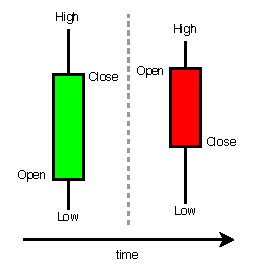
\includegraphics{candlesticks}
			\caption{Example of a rising (left) and a falling
				(right) japanese candlestick, commonly used in
				trading to aggregate market
				data.}\label{fig:candlesticks}
		\end{figure}
	\item[Volume] The amount traded during a \textit{trading day} in a
		\textit{market} by all the traders that operated in the market,
		expressed in terms of the \textit{base currency}.
	\item[Winning trade] A \textit{trade} concluded with a profit. In the
		case of a \textit{buy trade}, this means that the \textit{exit
		order} has sold the \textit{base currency} at an higher price
		than the one at which the base currency was bought in the
		\textit{entry order}. In the case of a \textit{sell trade}, this
		means that the exit order has bought the base currency at a
		lower price than the one at which the base currency was sold in
		the entry order.
\end{description}
